\label{sec:neuro_expl}

In this thesis, concepts specific to neuromorphic engineering will be used extensively.
Before diving into the design and results of the proposed controllers, a clear understanding of these and other related concepts must be achieved.
Otherwise, comprehension of the choices or design decisions will be difficult.

\section{Excitability}

The first step in understanding neuronal systems is the concept of excitability. 
In the words of \citet{excDef}, \enquote{Excitability is the property of a system to exhibit all-or-none response to pulse inputs}. 
In other words, the system does not react to pulses until the pulse amplitude and/or length crosses a certain threshold after which the system responds completely. 

In \cref{fig:excitability}, an example of an excitable behavior is displayed. 
As can be seen, a very small difference in the pulse amplitude resulted in a very different neuronal behavior. 
The lower pulse resulted in the output faithfully following the input while the output of the higher one exhibited a very different behavior with oscillation and  peaks far above the input. 
The second behavior is known as "bursting" and will be discussed later.
Also, this example highlights that the "none" response does not need to be a complete silence but can be a simple linear response to the input. 
This is the behavior exhibited by the neuronal model of this thesis.

\begin{figure}[htb]
    \centering
    \inserttikzfig{plots/excitability.tikz}
    \caption{Example of an excitable behavior. Generated using neuron model of \cref{sec:model}.}
    \label{fig:excitability}
\end{figure}

Most neuronal systems contain some excitable blocks such as neurons. 
Indeed, on a conceptual level, the all-or-none response is important for transforming continuous input into discrete events. 
This discretization makes a system more resilient to noise and capable of reacting only when necessary.

This kind of response is desired in our controller because effective control of the oscillation of a pendulum requires a very all-or-nothing control input.
Indeed, actuation should only occur at specific times. In addition, the moment of actuation is crucial when controlling a pendulum, and actuating at a bad time can lead to very poor results.
In the words of \citet{excDef}, \enquote{\textins{Excitability} is instrumental in converting sensory signals into motor actions}.

More theoretically, to create an excitable system, a localized positive feedback loop is necessary. 
Indeed, the switch between two different responses after crossing a threshold requires the activation of a positive feedback near the threshold. 
This feedback pushes the output of the system to generate the excitable event.
The locality of this positive feedback also prevents the output from growing to infinity.

\section{Conductance-based neuron models}

With excitability defined, neuronal models can be understood more clearly. Indeed, neurons are a prime example of an excitable system.

In the words of \citet{neurDef}, \enquote{Neurons are the basic building blocks of the nervous system, which includes the brain, the spinal cord, and the peripheral nervous system. These specialized cells are the information-processing units responsible for receiving, processing, and transmitting information by electrical and chemical signaling.}.

In other words, neurons are cells that can receive input from the external world, send messages to one another, and send motor commands to muscles.  The relationship between the input received and the commands or messages sent is the processing performed by the neuron. Because neurons can be relatively large compared with the scale of electrical or chemical signaling, it is evident that their behavior may be different in different parts of the cell. However, a common way to observe a neuron is to measure and model its activity in only one location. This leads to the neuron being seen as a block with a single input and output and a certain hidden state.

As shown by \citet{neuronIons}, the state of a neuron at its axon membrane can be described by the flow of ionic currents. The magnitude of these currents is determined by the potential across the interior and exterior of the cell, which opens or closes channels at different speeds depending on the channel type. In turn, these currents flowing into or out of the cell influence the potential across the interior and exterior of the cell. 

This model is illustrated on \cref{fig:conductance_neuron}, where ionic currents flow through channels in the neuron membrane. Some of these channels activate and deactivate based on the membrane potential. Other are influenced by other factors such as the activity of other neurons or changes in biochemistry.

\begin{figure}[htb]
    \centering
    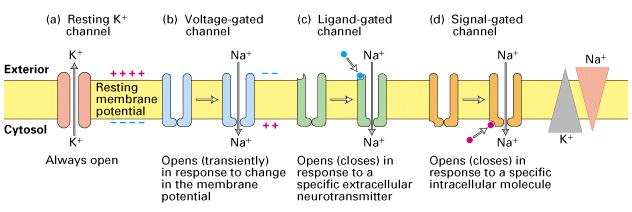
\includegraphics[width=.9\textwidth]{channels.png}
    \caption{Simplified diagram of a biological neuron membrane. (Diagram taken from \citet{channelDiagram})}
    \label{fig:conductance_neuron}
\end{figure}

\begin{figure}[htb]
    \centering
    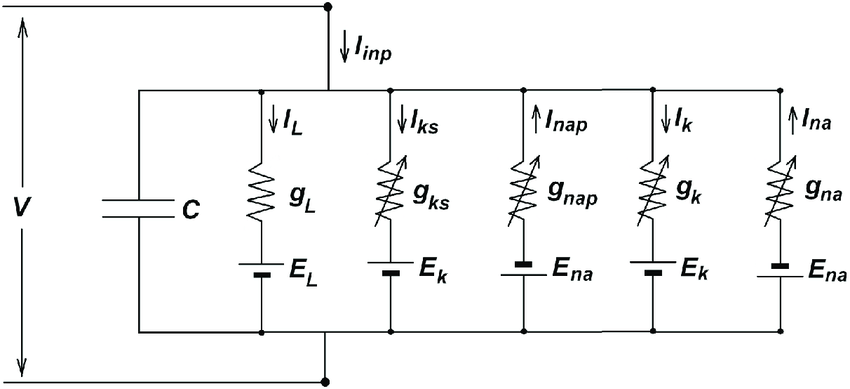
\includegraphics[width=.9\textwidth]{conductanceNet.png}
    \caption{Simplified circuit of the neuron model. (Circuit taken from \citet{electricDiagram})}
    \label{fig:conductance_neuron_circuit}
\end{figure}

This language of currents and potentials seems to designate classical circuit theory as the most useful tool to model the behavior of a neuron.
\citet{conductanceModel} were the first to formulate a model of neuronal behavior using a parallel network of dynamic conductances.
These conductances change based on the membrane voltage of the neuron at different rates, mimicking the opening and closing of the channels.
A good representation of this model is seen in \cref{fig:conductance_neuron_circuit}.
On this diagram, it can be seen that some ionic current discharge the capacity that represents the membrane while others charge it.
Those charging currents effectively act as positive feedback loops.
As seen in the previous section, these are necessary for the excitable behavior of a neuron.

Using circuit theory, this model can be written more formally using ordinary differential equation. 
\Crefrange{eq:hodgkinstart}{eq:hodgkinend} are a very general representation of this model.
In this representation the $i$ subscripts denote the different ionic currents that can be found in \cref{fig:conductance_neuron_circuit}.

\begin{align}
    C\frac{\partial V}{\partial t} =& I_\text{inp} - g_L\left(V-E_L\right) - \sum_i I_i\label{eq:hodgkinstart}\\
    I_i\left(t, V\right) =& g_i\left(t, V\right)\left(V - E_i\right)\\
    g_i\left(t, V\right) =& \bar{g_i}m_i\left(t, V\right)^{p_i} h_i\left(t, V\right)^{q_i}\\
    \frac{\partial m_i\left(t, V\right)}{\partial t} =& \frac{m_{i\infty}\left(V\right) - m_i\left(t, V\right)}{\tau_{mi}\left(V\right)}\\
    \frac{\partial h_i\left(t, V\right)}{\partial t} =& \frac{h_{i\infty}\left(V\right) - h_i\left(t, V\right)}{\tau_{hi}\left(V\right)}\label{eq:hodgkinend}
\end{align}

The $m_\infty$, $h_\infty$, $\tau_m$ and $\tau_h$ functions are saturation functions. 
The saturation of the $\infty$ terms show that the ionic current feedbacks are localized in a certain range of membrane voltage.

The $m_\infty$ are increasing positive saturation functions, while the $h_\infty$ are decreasing positive saturation functions.

In this case, what is important for feedback is the local feedback, which is characterized by the differential conductance.
Studying the global feedback would be useless since a conductance is a passive element and it always acts as a global negative feedback. 
The range of the saturation of $m_\infty$, $h_\infty$ and the power assigned to them will determine where the term acts as positive feedback and when it acts as a negative feedback.

This model is very general , and when parameters are chosen properly, it can generate a whole range of neuronal behaviors seen in biological neurons.
However, it is very hard to tune, and small changes in parameters can completely change the behavior of the system, whereas large changes may leave the output looking identical.
This is important in a biological system to improve robustness to variations while providing efficient switching between modes.
But, in this thesis, all these advantages are of very little use.
Therefore, a simplified model will be used to make tuning easier.

In this thesis, only spiking and bursting, the two most common behaviors, will be used; therefore, only these behaviors will be studied. These two behaviors can be seen in \cref{fig:behaviors}.
A spike is a sudden, short, and steep increase in the membrane voltage followed by a sharp decrease and return to a resting voltage. 
A burst is the apparition of a packet of spikes.
A spike is a prime example of the importance of fast local positive feedback. 
Indeed, a spike is formed by the positive feedback pushing the voltage of the neuron upward before deactivating and letting the slower negative feedback drag down the voltage before the positive feedback reactivating in the other way to push the voltage downward.

Classically, both behaviors can be classified as tonic or phasic.
A tonic response means that the response persists as long as the stimulus is maintained.
This is observed in \cref{fig:behaviors} where the spike and burst repeat.
A phasic response means that the response is localized at the apparition of the stimulus and will fade as the stimulus is maintained. 
This is observed in \cref{fig:excitability}, the burst does not continue after the initial response.
Often, for a set of parameters, as the input current increases, a neuron will first have a phasic response before starting to become tonic.
% Tonic or not tonic bursting and spiking

\begin{figure}[htb]
    \centering
    \inserttikzfig{plots/neuron_behaviour.tikz}
    \caption{Example of spiking and bursting behaviors. Generated using the neuron model of \cref{sec:model}.}
    \label{fig:behaviors}
\end{figure}

\section{Neuronal Behavior Metrics}

The previous section introduced the spiking and bursting behaviors. 
These behaviors are highly complex and therefore, to be able to compare different bursting or spiking realizations, multiple specific metrics must be defined.
Here, only the metrics to evaluate the tonic spiking and the tonic bursting will be discussed.
It is easy to derive similar metrics for the phasic case.

To compare different bursting realizations, it is important to consider the shape of a burst and the link between two bursts.
\Cref{fig:burst_metrics} represents values that can be directly inferred from the trance of a tonic bursting neuron that are enough to characterize a specific bursting trace.
These values can be defined as
\begin{description}
    \item[Burst length] Average time of a burst event.
    \item[Rest length] Average time of inactivity between two burst events.
    \item[Burst period] Average time between the start of two burst events.
    \item[Spike period] Inside a burst, the average time between the start of two spike events.
    \item[Number of spikes] Average number of spikes inside a burst event.
\end{description}

\begin{figure}[htb]
    \centering
    \inserttikzfig{diagrams/burst_metrics.tikz}
    \caption{Illustration of the different metrics used to describe bursting. Generated using the neuron model of \cref{sec:model}.}
    \label{fig:burst_metrics}
\end{figure}

Aside from the number of spikes, these raw metrics are not the most telling.
Instead, the following set of metrics derived from the aforementioned values is used.
\begin{description}
    \item[Inter-burst frequency] $\frac{1}{\text{Burst period}}$, the frequency at which burst events occur.
    \item[Intra-burst frequency] $\frac{1}{\text{Spike period}}$, frequency at which spikes occur inside a burst event.
    \item[Duty cycle] $\frac{\text{Burst length}}{\text{Burst period}}$, the portion of a period during which the neuron is inside a burst event.
    \item[Number of spikes] Average number of spikes inside a burst event.
\end{description}
Even though the inter-burst and intra-burst frequencies are just the inverses of direct metrics, the realm of frequencies is often better suited for comparison between realizations

On the other hand, spiking is simpler and does not require as many metrics.
The only direct metric is measuring the \textbf{Spike period}.
It is sufficient to compute the \textbf{Spiking frequency} , which is the most useful metric for describing spiking behavior. 
For the same reason as the bursting transformation to the frequency realm is better for comparison.

\section{Central Pattern Generators and Rhythms}

From \citet{cpgDef}, \enquote{A central pattern generator (CPG) is an assembly of neurons that can produce a rhythmic activity pattern without \textdel{phasic} sensory feedback information}.
This construction thus uses multiple neurons to generate a certain rhythm.

It is widely accepted that central pattern generators (CPGs) are frequently found in biological motion systems.
\citet{cpgMotion, cpgMotion2} highlight that CPGs are abundant in animals for motion control.
The natural periodic oscillations of CPGs makes them easier to pair them with systems that are already periodic.

Therefore, the concept of central pattern generators (CPGs) is very useful for developing controllers.
Indeed, CPGs being closely linked to rhythmic movements pair well with the naturally rhythmic movement of the oscillation of a pendulum.

Here, to keep it simple, the connections between neurons inside a CPG result in the activity of the presynaptic neuron generating currents in the postsynaptic neuron.
These connections can have two types, inhibitory and excitatory.
Inhibitory connection results in a negative current being injected, whereas excitatory connection results in a positive current.

As an example, one of the most simple and well-studied CPGs is the half-center oscillator \citep{halfcenter}.
This specific circuit is composed of two neurons that inhibit each other.
The system along with a simulation can be seen in \ref{fig:halfcenter}.
The dents in the activity of one neuron appearing when the other is active highlight that currents flow from one neuron to the other only if the presynaptic neuron is activated. 

\begin{figure}[htb]
    \centering
    \inserttikzfig{diagrams/halfcenter.tikz}
    \caption{Example of an half center oscillator. Traces were generated using neuron model of \cref{sec:model}.}
    \label{fig:halfcenter}
\end{figure}

The generation of rhythmic patterns is clear when looking at the traces of the activation of both neurons.
Indeed, the activation of neurons 1 and 2 always follow each other.

The interesting aspect of CPGs is that the network may be able to generate a rhythm while an individual neuron may be silent.
This shows that the structure of the CPG is instrumental and is the key factor in the qualitative rhythm produced.
Very different models of neurons will still generate the same rhythm when used in a fixed CPG structure.
%This temporal shift can be expressed in term of phase by saying that one neuron as a phase of $\frac{1}{2}$ of a period compared to the other.
% Cite marder or other of different CPGs, show graphs of rythms

\section{Embodied Intelligence and CPGs} 

From \citet{embodiedDef} \enquote{Embodied intelligence is the computational approach to the design and understanding of intelligent behavior in embodied and situated agents through the consideration of the strict coupling between the agent and its environment (situatedness), mediated by the constraints of the agent’s own body, perceptual and motor system, and brain (embodiment).}.

This concept describes the goal of this thesis.
Indeed, the model developed later is a prime example of embodied intelligence.
The controller processes the direct sensory input to generate coherent control signals for the motor. 
Using neuromodulation, the strength of the push is changed according to the desired amplitude.
This amounts to intelligent behavior generated by components directly interacting with sensors and motors.

More broadly, the concept of embodied intelligence is closely related to CPGs.
Indeed, CPGs are circuits that are rhythmic without sensory feedback, but using sensory feedback to tune the frequency of the CPG to the external is thought to be the inner working of most biological motion controllers (citation needed).
This coupling is precisely a low-level embodied intelligence.

To simplify embodied intelligence, it can be seen as the coupling of sensing computing and actuating.
The agent in embodied learning has sensors, computing, and actuation in the same body.
% Define embodied Intelligence and its relationship with CPGs 
